

\chapter{Numerical Solution of Drift-Diffusion and Poisson's Equation} % Main chapter title

\label{Chapter3} % Change X to a consecutive number; for referencing this chapter elsewhere, use \ref{ChapterX}

\lhead{Chapter 3. \emph{Numerical Solution for Drift-Diffusion Equations}} % Change X to a consecutive number; this is for the header on each page - perhaps a shortened title
\begin{doublespace}


The simulation method developed in this thesis requires certain properties ,such as limitation of particle density or a combination of 1-D and 2-D simulations, which are not normally available in most commercial simulators. It is also possible that other unusual properties that are not studied in this thesis will be needed for further research. In this chapter a method for solving drift diffusion equations as well as Poisson's equation are developed based on finite difference method. This fully functioning simulator will have the needed flexibility for current and future research opportunities.  


\section{Finite Difference Method}
There are many different methods that can be used to solve drift diffusion equations such as finite elements, finite difference or meshless methods. Finite difference was chosen as an appropriate method for this thesis due to its simplicity which allows straightforward implementation of unusual physical properties. Finite difference uses an approximation for the derivative of a function based on the mathematical definition of the derivative\cite{numerical2}.

\begin{equation}
\frac{df}{dx}=\lim\limits_{h \rightarrow 0} \frac{f(x+h)-f(x)}{h}
\end{equation}

It is possible to obtain a numerical approximation for the first derivative of a function by dropping the limit and assuming that h is small enough that the numerical derivative is reasonably close to the actual derivative. As h gets smaller the approximation becomes more and more accurate. The difference between the calculated value and the real value is called the truncation error and it is captured using $O(h^n)$ notation. n signifies the order of h which determines how fast the approximation is approaching the real solution as h decreases\cite{numerical2}.  
\begin{equation}
\frac{df}{dx}=\frac{f(x+h)-f(x)}{h} + O(h)
\label{numdif}
\end{equation}

It is possible to uniformly discretize the entire region over which a function is defined in order to calculate its derivative. The first step is the division of the region over which the function is defined into \textit{n-1} segments. This creates \textit{n} number of points. Then the length of each segment is defined using the following relationship:

\begin{equation}
h=\frac{L}{n}
\end{equation}

A function is defined at the edge of every segment. All the points can be labeled consecutively, $x_0,x_1,x_2$ ... $x_{n-1}$ where $x_i=ih$. The function is discretely defined on \textit{$f_{i}=f(x_{i})$} where\textit{ i=0,1,2..n-1}. It is possible to use equation  \ref{numdif} to discretely calculate the first derivative of the function with respect to x.

\begin{equation}
\frac{df(x_i)}{dx}=\frac{f(x_{i+1})-f(x_i)}{h} + O(h)
\end{equation}
Above equation is called forward difference because the derivative for point $x_i$ was calculated using the point that is coming right after it, $x_{i+1}$.
\begin{equation}
f^{'}_i=\frac{f_{i+1}-f_i}{h}+ O(h)
\end{equation}

Forward difference is not the only way to calculate a numerical derivative. Here are a couple other ways calculate the same derivative by using different points.

\begin{equation}
f^{'}_i=\frac{f_{i}-f_{i-1}}{h}+ O(h)
\label{bdif}
\end{equation}

\begin{equation}
f^{'}_{i+\frac{1}{2}}=\frac{f_{i+1}-f_i}{h}+ O(h^2)
\label{cdif}
\end{equation}

Equation \ref{bdif} is called backward difference and equation \ref{cdif} is called central difference. One important aspect to note here is that in the central difference formula the derivative falls exactly in the middle of two points. It also gives more accurate results using the same number of points as forward and backward difference. 

Using finite difference formulas it is possible to construct higher order derivatives. A formula for a second order derivative at point $x_i$ using central difference can be calculated using a first order derivative on $x_{i-\frac{1}{2}}$, $x_i$ and $x_{i+\frac{1}{2}}$  

\begin{equation}
f_{i+\frac{1}{2}}^{'}=\frac{f_{i+1}-f_{i}}{h}
\label{forwardd}
\end{equation}

\begin{equation}
f_{i-\frac{1}{2}}^{'}=\frac{f_{i}-f_{i-1}}{h}
\label{backwardd}
\end{equation}

\begin{equation}
f^{'}_{i}=\frac{f_{i+\frac{1}{2}}-f_{i-\frac{1}{2}}}{h}
\label{2ndord}
\end{equation}

The second order derivative is constructed by taking the second derivative of the last function. Then equations \ref{forwardd} and \ref{backwardd} are placed into \ref{2ndord}.

\begin{equation}\nonumber
f^{''}_{i}=\frac{f_{i+\frac{1}{2}}^{'}-f_{i-\frac{1}{2}}^{'}}{h}
\end{equation}

\begin{equation}\nonumber
f^{''}_{i}=\frac{\frac{f_{i+1}-f_{i}}{h}-\frac{f_{i}-f_{i-1}}{h}}{h}
\end{equation}

\begin{equation}\nonumber
f^{''}_{i}=\frac{f_{i+1}-f_{i}-f_{i}+f_{i-1}}{h^2}
\end{equation}

Second order derivative takes the following form:

\begin{equation}
f^{''}_{i}=\frac{f_{i+1}-2f_{i}+f_{i-1}}{h^2}+O(h^2)
\label{fdc2}
\end{equation}

Overall these finite difference equations are enough to solve drift diffusion equations. Even though all the derivations are done in 1-D it is trivial to extend them to other dimensions. This method can be used to solve Poisson's equation and drift diffusion equations.

\clearpage

\section{Poisson Solver}

Poisson's equation needs to be solved before drift diffusion equations in order find the potential distribution as well as the electric field inside the device. In order to solve for the electric field and the potential, Poisson's equation is simplified through assumptions and then the finite difference method is used to solve this simplified equation\cite{smith1985numerical}. The first step of simplification is assuming that the permittivity is isotropic.
 
\begin{equation}
\nabla \cdot  (\varepsilon \nabla V)=-\rho
\end{equation}

\begin{equation}
\nabla \cdot  (\varepsilon \nabla V)=\varepsilon  \nabla^2 V
\end{equation}

Dividing both sides by permittivity and expanding the left hand side,,

\begin{equation}
 \nabla^2 V =-\frac{\rho}{\varepsilon}
 \label{Poissons}
\end{equation}

\begin{equation}
 \nabla^2 V =\frac{\partial^2 V}{\partial^2 x}+\frac{\partial^2 V}{\partial^2 y}
\end{equation}

After discretizing the electric potential over a uniform 2-D grid and using the second order central finite difference formula \eqref{fdc2} laplacian of the electric potential can be calculated using\cite{NumModel}:

\begin{equation}
 \nabla^2 V_{i,j}=\frac{V_{i+1,j}-2V_{i,j}+V_{i-1,j}}{\Delta x^2}+\frac{V_{i,j+1}-2V_{i,j}+V_{i,j-1}}{\Delta y^2}
 \label{nablafd}
\end{equation}

Since the grid is uniform the distance between two nodes in x and y directions are equal therefore only one variable is needed to represent the distance between two points.

\begin{equation}
\Delta=\Delta x =\Delta y
\label{delta}
\end{equation}

Net charge density and the permittivity is also discretized over the same uniform mesh. Discretized form of Poisson's equation is generated by combining equations \ref{Poissons} ,\ref{nablafd} and \ref{delta}.

\begin{equation}
 \nabla^2 V_{i,j}=\frac{V_{i-1,j}+V_{i,j-1}-4V_{i,j}+V_{i+1,j}+V_{i,j+1}}{\Delta^2}=-\frac{\rho_{i,j}}{\varepsilon_{i,j}}
\end{equation}

This equation can be rearranged into the form below:
\begin{equation}
\varepsilon_{i,j}(V_{i-1,j}+V_{i,j-1}-4V_{i,j}+V_{i+1,j}+V_{i,j+1})=-\Delta^2\rho_{i,j}
\label{discrete_poisson}
\end{equation}



Combining the equations above (\ref{discrete_poisson}, \ref{dirichlet}, \ref{neumannx} and \ref{neumanny}) it is possible to turn Poisson's equation, which is a second order differential equation, into a linear set of coupled algebraic equation.

\begin{equation}
D_{2}\vec{V}=-\Delta^2\vec{\rho}-\vec{V_b}
\end{equation}

$D_{2}$ is the Laplace operator converted into a matrix using the finite difference method. One can easily get the potential distribution by simply solving this matrix equation(\ref{poimatrix}). Due to the nature of the problem the resulting matrix is quite sparse and using a sparse LU rather than a regular LU decomposition increases the computational efficiency. Additionally, LU decomposition only needs to be performed once since the equation is static and L and U matrices can be reused for all the solutions following the initial one. 

\begin{equation}
\vec{V}=D_{2}^{-1}(-\Delta^2\vec{\rho_{i,j}}-\vec{V_b})
\label{poimatrix}
\end{equation}

After solving for the potential distribution it is straightforward to calculate the electric field distribution discretely by using the relationship between the electric field and the electric potential \eqref{Efield} and the central difference equation \eqref{cdif}. 

\begin{equation}
\vec{E^x_{i,j}}=-\frac{V_{i+1,j}-V_{i-1,j}}{2\Delta}
\end{equation}

\begin{equation}
\vec{E^x_{i,j}}=-\frac{V_{i,j+1}-V_{i,j-1}}{2\Delta}
\end{equation}

\clearpage
\section{Current Density Equations}
 Both drift and diffusion currents can be calculated over the entire grid. Drift current does not involve any differentials but it is a function of the electric field and the diffusion current can be calculated using first order central difference\cite{Dragica1}. The current density is calculated in such a way that it falls between two points which simplifies the application of the boundary conditions.
\begin{equation}
J^x_{i+\frac{1}{2},j,k}=q\mu_n n_{i+\frac{1}{2},j,k} E^x_{i+\frac{1}{2},j,k}+q D_n \frac{n_{i+1,j,k}-n_{i,j,k}}{\Delta}
\end{equation}
The electric field is calculated exactly on the nodes and linear interpolation is used in order to get a value between the nodes. The same argument is also valid for particle densities \textit{p} and \textit{n}. They are defined at the nodes but they are linearly interpolated to be used in current density equations.

\begin{equation}\nonumber
n_{i+\frac{1}{2},j,k}=\frac{n_{i+1,j,k}+n_{i,j,k}}{2}
\end{equation}
\begin{equation}\nonumber
E^{x}_{i+\frac{1}{2},j,k}=\frac{E^y_{i+1,j,k}+E^y_{i,j,k}}{2}
\end{equation}

Current density in y direction is calculated by following the same method:

\begin{equation}
J^y_{i,j+\frac{1}{2},k}=q\mu_n n_{i,j+\frac{1}{2},k} E^y_{i,j+\frac{1}{2},k}+D_n \frac{n_{i,j+1,k}-n_{i,j,k}}{\Delta}
\end{equation}
\begin{equation}\nonumber
n_{i,j+\frac{1}{2},k}=\frac{n_{i,j+1,k}+n_{i,j,k}}{2}
\end{equation}
\begin{equation}\nonumber
E^{y}_{i,j+\frac{1}{2},k}=\frac{E^y_{i,j+1,k}+E^y_{i,j,k}}{2}
\end{equation}


\clearpage
\subsection{Continuity Equation}
The continuity equation is needed to calculate a transient solution for the drift diffusion equations. The equation is simple to discretize using the finite difference method. There are two terms that need to be discretized, a first order derivative in time and a first order derivative in space. First the divergence term in the equation \eqref{conn} needs to be evaluated.

\begin{equation}
\nabla \cdot J=\frac{\partial J}{\partial x}+\frac{\partial J}{\partial y}=\frac{d J_x}{d x}+\frac{d J_y}{d y}
\end{equation}

It is possible to replace the derivative with central finite difference terms.
\begin{equation}
\frac{d J_x}{d x}=\frac{J^x_{i+\frac{1}{2},j,k}-J^x_{i-\frac{1}{2},j,k}}{h}
\end{equation}
\begin{equation}
\frac{d J_y}{d y}=\frac{J^y_{i,j+\frac{1}{2},k}-J^y_{i,j-\frac{1}{2},k}}{h}
\end{equation}
\begin{equation}
\nabla \cdot J_{i,j,k}=\frac{J^x_{i+\frac{1}{2},j,k}-J^x_{i-\frac{1}{2},j,k}}{h}+\frac{J^y_{i,j+\frac{1}{2},k}-J^y_{i,j-\frac{1}{2},k}}{h}
\label{delJ}
\end{equation}

This is the general form of the divergence of the current density. These set of equations can be placed into a matrix which is a linear function of particle density at time t.

\begin{equation}
B = \nabla \cdot J_k 
\label{fd_div}
\end{equation}

The time derivative can be replaced by a forward or a backward finite difference term respectively.

\begin{equation}
\frac{\partial  \vec{n}_k}{\partial t}=\frac{ \vec{n}_{k+1}-\vec{n}_k}{\Delta t}
\label{forwardtime}
\end{equation}

\begin{equation}
\frac{\partial \vec{n}_k}{\partial t}=\frac{ \vec{n}_k- \vec{n}_{k-1}}{\Delta t}
\label{backwardtime}
\end{equation}

It is possible to find a numerical transient solution for the drift-diffusion problem by combining finite difference form of the time derivative (\eqref{forwardtime} or \eqref{backwardtime}) and the divergence of the current density equations \eqref{fd_div}.

Forward difference approximation can be used to get an explicit solution for the continuity equation\cite{Dragica1}.

\begin{equation}\nonumber
\frac{ \vec{n}_{k+1}-\vec{n_k}}{\Delta t}=B
\end{equation}

\begin{equation}
\vec{n}_{k+1}=\vec{n_{k}}+\Delta t B
\label{explicit}
\end{equation}

Both forward and backward difference formulas work sequentially in order to generate a transient solution. The solution from the previous time step is needed to calculate the solution for the next time step. The forward difference gives an explicit solution which has a few advantages. This solution can be implemented, without forming any matrices by directly calculating the divergence of the current density for each node and then marching through time using equation \ref{explicit}. Additionally, unlike backward difference, there are no equations to be solved for every time step. These two properties ease the computational load of the problem and speed up the solution process. Unfortunately this scheme has stability conditions which have to be met in order to produce a solution\cite{Dragica1}.

Backward difference can be replaced by forward difference to get an implicit solution.
\begin{equation}\nonumber
\frac{ \vec{n}_{k}-\vec{n}_{k-1}}{\Delta t}=\frac{1}{q}(qB)
\end{equation}
\begin{equation}\nonumber
\vec{n}_{k}-\Delta t B =\vec{n}_{k-1}
\end{equation}

Since all the equations in B matrix are a linear functions on n, it can be separated into two terms, $B=Cn$.
\begin{equation}\nonumber
\vec{n}_{k}-\Delta t C\vec{n}_{k-1} =\vec{n}_{k-1}
\end{equation}
\begin{equation}
\vec{n}_k=(I-\Delta t C)^{-1}\vec{n}_{k-1}
\end{equation}

This solution needs a matrix inversion every time step but it is unconditionally stable\cite{Dragica1} as long as it is not coupled with Poisson's equation. The decision to use an implicit or an explicit solution requires deliberate analysis and it will be discussed in detail in the section 3.4.
\clearpage

\section{Stability and Computational Efficiency}
Before discussing  the numerical limitations of solving the drift diffusion equation via finite difference it is important to look into the physical limitations of the problem. These limitations persist no matter what kind of numerical scheme is employed to solve the drift diffusion equation.

\subsection{Physical Limitations}
Debye length is the length over which mobile charge carriers screen out an external electric field and it determines how steeply charges will accumulate over a certain distance.
\begin{equation}
L_D=\sqrt{\frac{\varepsilon V_{th}}{q n}}
\label{debye}
\end{equation}
Debye length limits how coarse the grid can be since the distribution of the charge density needs to be accurately captured. As it can be seen from the formula above the higher the charge density is the steeper the charge will accumulate. This behavior is also appears in the analytic solution provided in section 2.2.1 in chapter 2. The accumulation of the charged particle at the wall becomes steeper as the electric field strength increases. The debye length can become a major problem for large devices with high charge densities since the mesh density needs to be extremely high.

The amount of time it takes for charge fluctuations to disappear is called Dielectric relaxation time. It limits the maximum time step of a simulation since the fluctuations that are not properly resolved over time will make the simulation unstable.

\begin{equation}
t_{dr}=\frac{\varepsilon}{q n \mu}
\label{tdr}
\end{equation}

Dielectric relaxation time is only important when the electric potential is significantly affected by the redistribution of charge over time. Otherwise it has minimal impact on the stability of the problem.
\subsection{Numerical Limitations}

There are also numerical limits which can affect convergence and stability of a solution when using an explicit finite difference scheme. These are called Courant-Friedrichs-Lewy (CFL)conditions \cite{NumModel}. CFL conditions for diffusion and drift are shown in the following equations.

\begin{equation}
\frac{\Delta ^2}{2 D_n}>\Delta t
\label{CFL_Diff}
\end{equation}

Above condition is for only diffusion and it restricts the maximum time step. The following condition is for drift dominated systems:

\begin{equation}
\frac{2 \Delta }{\mu E}>\Delta t
\label{CFL_Drift}
\end{equation}

This is the second numerical restriction on the simulation. The condition for drift depends on the electric field therefore it needs to be satisfied at all times as the electric field changes over time during simulation.

Both physical and numerical constraints have to be evaluated and mesh density and time step need to be selected in order to satisfy all these conditions discussed above. Particularly mesh density has a very strong impact on the accuracy, stability and the computational efficiency of the simulation. Increasing the mesh density increases the computational time needed to calculate every time step since there are more operations to be performed. Additionally because of the CFL condition for diffusion, the time step is related to the square of the mesh size. This means that maximum allowed step size decreases much quicker than the mesh density. Also, increasing charge density can decrease the maximum mesh size to a very small value. This can be improved by using a non uniform mesh which can dramatically decrease the number points needed for the simulation. This is usually not very straightforward to implement in a finite difference scheme and a small mesh size requires small time steps. This cannot be avoided through non uniform meshing. Both numerical and physical constraints for the memristor simulation are further discussed in chapter 5.

\subsection{Explicit vs. Implicit Solution}

Overall explicit and implicit solutions have their advantages and disadvantages. Choosing one over the other requires a careful analysis of the problem. Implicit solution by itself is unconditionally stable therefore it can support very large time steps without any stability issues. However, the accuracy of the transient solution decreases with a larger time step but the steady state solution is not affected. So for steady state solutions it is better to use an implicit method which can reach steady state very quickly. This advantage disappears when the particle densities are high enough to affect the electric field and Poisson's equation needs to be solved for every time step. In this scenario the maximum time step is determined by the dielectric relaxation time which can be around the same order as CFL conditions or even smaller. Since the time step is going to be around the same order for both implicit and explicit methods it is reasonable to use the explicit solution because it is computationally less expensive.

Usually an implicit solution is preferable when there is no coupling between Poisson's equation and the drift diffusion equations and the transient response is not very important. Explicit solution has an edge over the implicit solution due to its lower computational requirements when the equations are coupled and the time steps for both schemes are restricted to small values. For memirstor simulation, the drift diffusion equations are strongly coupled with Poisson's equation. For this reason all the memristor simulations in this thesis use explicit time stepping. 


\clearpage
\section{Simulation Procedure}
The different equations and schemes that were used to solve the drift diffusion  and Poison's equation have been presented over the past few sections. Using all this information it is possible create a general approach to solve a drift diffusion problem. The geometry and the physical properties of the problem as well as all the initial and the boundary conditions need to be defined at the beginning of the solution process. The initialization sets up the first time step of the problem at $t=0$. Once this first step is done it is possible generate the required vectors and matrices and solve the problem for the next time steps, $t=t_i$. 

The solution process starts by solving Poisson's equation using the charge distribution at current time step. Once it is solved, the electric field distribution is calculated and used in the drift diffusion equations to calculate the current density distribution. Explicit time stepping is used to determine the carrier density in the next time step. Finally once the carrier distribution for the next step is calculated it is possible check for a stopping criterion. If this criterion is not met then the whole process will start all over again. If the charge concentration is so small that the equations are decoupled then it is possible to skip solving Poisson's equation for the rest of the simulation which speeds up the solution process.

 There are two different criteria that can be used to decide whether to finalize the simulation process or not. The simulation can stop if it reaches a certain point in time. This is quite simple since the current time can be checked and if it is equal or greater than the required simulation time then the simulation can be stopped. It is also possible to simulate until the simulation reaches steady state. This can be determined by comparing the current carrier distributions with distribution at the previous time step. If the difference is very small then the time derivatives of the carrier densities are very close to zero and the simulation has reached steady state therefore the simulation process can be stopped. The flowchart in figure \ref{flowchart} summarizes the solution procedure.

\clearpage

\begin{figure}
\centering
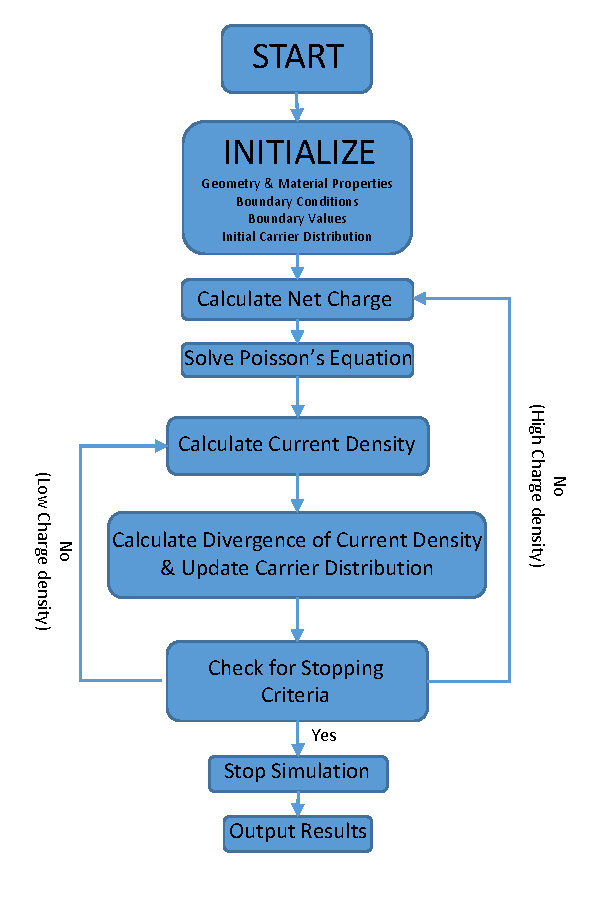
\includegraphics[scale=1.3]{flowchart}
\caption{Finite Difference Drift-Diffusion Scheme Flowchart} 
\label{flowchart}
\end{figure}


\end{doublespace}
